
\begin{figure}[ht]
\centering
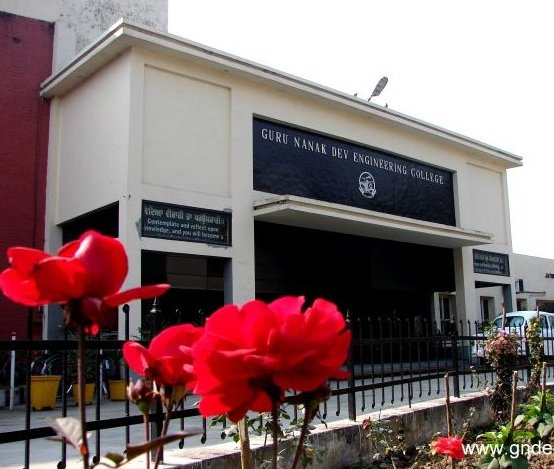
\includegraphics[scale=0.5]{input/images/gndec.jpg}
\caption{Guru Nanak Dev Engineering College}
\end{figure}
\hspace{-1.7em}
 Guru Nanak Dev Engineering College was established by the Nankana Sahib Education Trust Ludhiana. The Nankana Sahib Education Trust i.e NSET
was founded in memory of the most sacred temple of Sri Nankana Sahib, birth place
of Sri Guru Nanak Dev Ji. With the mission of Removal of Economic Backwardness
through Technology Shiromani Gurudwara Parbandhak Committee i.e SGPC started a
Poly technical was started in 1953 and Guru Nanak Dev Engineering College was established in 1956.\\
NSET resolved to uplift Rural areas by admitting 70\% 
of students from these rural
areas ever year. This commitment was made to nation on 8th April, 1956, the day
foundation stone of the college building was laid by Dr. Rajendra Prasad Ji, the First
President of India. The College is now ISO 9001:2000 certified.\\
Guru Nanak Dev Engineering College campus is spread over 88 acres of prime land
about 5 Kms from Bus Stand and 8 Kms from Ludhiana Railway Station on Ludhiana-Malerkotla Road. The college campus is well planned with beautifully laid out tree plantation, pathways, flowerbeds besides the well maintained sprawling lawns all around. It
has beautiful building for College,Hostels,Swimming Pool,Sports and Gymnasium Hall
Complex, Gurudwara Sahib, Bank, Dispensary, Post Office etc. There are two hostels
for boys and one for girls with total accommodation of about 550 students. The main
goal of this institute is:\\
\begin{itemize}
\item To build and promote teams of experts in the upcoming specialisations.
\item To promote quality research and undertake research projects keeping in view their relevance to needs and requirements of technology in local industry.
\item To achieve total financial independence.
\item To start online transfer of knowledge in appropriate technology by means of establishing multipurpose resource centres.
\end{itemize}


